% Standalone editable source. Compile twice with pdfLaTeX.
% Earlier Mermaid companions are not synchronized with this revision.
\documentclass[11pt,a4paper]{article}
\usepackage[T1]{fontenc}
\usepackage[utf8]{inputenc}
\usepackage{lmodern,microtype,amsmath,amssymb,tabularx,array,booktabs}
\usepackage[margin=20mm,headheight=14pt]{geometry}
\usepackage{xcolor,tikz,fancyhdr,hyperref}
\usetikzlibrary{arrows.meta,positioning,shapes.geometric}
\definecolor{ink}{HTML}{17324D}\definecolor{teal}{HTML}{127D83}\definecolor{pale}{HTML}{EDF5F5}
\hypersetup{colorlinks=true,linkcolor=ink,pdftitle={From Reality to Ontology and Flow}}
\pagestyle{fancy}\fancyhf{}\fancyhead[L]{\small\textsc{ABM / Guide 0}}\fancyhead[R]{\small Constructing $O_0$}\fancyfoot[C]{\thepage}
\setlength{\parindent}{0pt}\setlength{\parskip}{6pt}
\renewcommand{\arraystretch}{1.15}
\newcommand{\st}[1]{\texttt{<<#1>>}}
\newcommand{\heading}[1]{\par\vspace{5pt}{\large\bfseries\color{ink}#1}\par}
\newcommand{\ruleline}{\par\vspace{2pt}\hrule\vspace{3pt}}
\tikzset{entity/.style={draw=ink,rounded corners=2pt,text width=36mm,align=left,inner sep=6pt,font=\small},lab/.style={font=\scriptsize,fill=white,inner sep=2pt,align=center},rel/.style={draw=ink,thick}}
% Entity content: #1 state visible, #2 methods visible.
\newcommand{\player}[2]{\st{agent}\\\textbf{Player}\ifnum#1=1\ruleline team\fi\ifnum#2=1\ruleline shoot()\\pass()\fi}
\newcommand{\field}[1]{\st{arena}\\\textbf{Field}\ifnum#1=1\ruleline limits\fi}
\newcommand{\ball}[1]{\st{artificiality}\\\textbf{Ball}\ifnum#1=1\ruleline playable\fi}
\newcommand{\referee}[2]{\st{artificiality}\\\textbf{Referee}\ifnum#1=1\ruleline currentScore\fi\ifnum#2=1\ruleline {\scriptsize\texttt{observeField()}}\\{\scriptsize\texttt{makeBallNotPlayable()}}\fi}
\newcommand{\rules}[1]{\st{artificiality}\\\textbf{SoccerRules}\ifnum#1=1\ruleline permittedActions\\endCondition\fi}
\newcommand{\inventory}[2]{\begin{center}\begin{tikzpicture}
\node[entity] at (-5,0) {\player{#1}{#2}};
\node[entity] at (0,0) {\field{#1}};
\node[entity] at (5,0) {\ball{#1}};
\node[entity,text width=43mm] at (-2.8,-3.3) {\referee{#1}{#2}};
\node[entity] at (3,-3.3) {\rules{#1}};
\end{tikzpicture}\end{center}}
\begin{document}
{\LARGE\bfseries\color{ink}From Reality to Ontology and Flow}\par
{\large Case: ``How to understand soccer''}

\heading{Our case and purpose}
We want to investigate \textbf{what causes one team to beat another in a soccer game}. Different theories could explain this: player abilities, coordination, tactics, or other factors. Implementing and comparing those theories will take time. The immediate homework task does not yet explain victory: it constructs and inspects a minimal representation of play. Today, we construct \textbf{$O_0$, our initial model ontology}: a first explicit statement of what our modeled soccer world contains.

\textbf{WHAT IS --- LUL:} entities, state, methods, and arrangements.\\
\textbf{HOW --- FC:} processes through which entities act, interact, and change.

We cannot explain how a team wins without first deciding what soccer is in our model. Modeling begins \emph{now}, with these representational decisions. Some will persist in later models; others will change as we learn.

\begin{quote}\large\bfseries Do not build the result into the model. Let it emerge from modeled actions and interactions.\end{quote}
We may give teams different characteristics to investigate their effects. We should not prescribe which team wins.

\heading{First, identify the Four As}
\textbf{A1 --- Agents.} Whose decision-making do we represent? Who can follow rules and, as the model develops, adapt?
\[A_1=\{\text{SoccerPlayer}\}.\]
\textbf{A2 --- Arena.} Where are agents situated, and what boundaries structure their environment?
\[A_2=\{\text{SoccerField}\}.\]
\textbf{A3 --- Artificiality.} What objects and institutional elements mediate action without separately modeled decision-making in this version?
\[
\begin{aligned}
A_{3m}&=\{\text{Ball}\},\\
A_{3s}&=\{\text{Referee-as-service},\text{SoccerRules}\}.
\end{aligned}
\]
The ball is material Artificiality; rules and the stipulated officiating service are social Artificiality. ``Referee'' below abbreviates this service: it has no separately modeled perception or discretionary judgment. An I-ABM can contain the artifacts and minimal social rules its question requires; it need not exclude Artificiality.
\textbf{A4 --- Array.} How are those elements arranged so that interaction, influence, observation, or transfer is possible?
\[
\begin{aligned}
A_4=\{&\text{player--ball interaction, player--field situatedness,}\\
&\text{ball--field containment, referee observation,}\\
&\text{rules applying to players and referee authority relations},\ldots\}.
\end{aligned}
\]
A1--A3 identify kinds of modeled elements, not individual instances. A4 organizes them into a system, including pairwise and higher-order configurations. SoccerRules and its prescriptions and permissions belong to $A_{3s}$. A4 specifies which entities those rules apply to and how authority, observation, and interaction are arranged. These categories are \emph{modeling roles}, not permanent properties of reality.

\newpage
\heading{Build one initial ontology, in four construction stages}
We use \textbf{LUL --- Light-UML-Like} to make our decisions visible. In diagrams, SoccerPlayer is abbreviated to Player and SoccerField to Field. As in Session 3, a class defines a type, objects are its instances, and methods describe available actions or operations. State includes attributes and their values. This class-level LUL omits object counts, inheritance, CLOCK, scheduling, software controllers, and emergent outcomes.
\[
O_{0a}\longrightarrow O_{0b}\longrightarrow O_{0c}\longrightarrow O_{0d}
\xrightarrow{\text{review and accept}}O_0.
\]
These are drafts of \emph{one} initial ontology. The final arrow marks a stopping decision, not necessarily another addition. Reserve $O_1,O_2,\ldots$ for substantive later revisions.

\heading{$O_{0a}$: draw the classes and identify their kind}
Draw the selected classes. Mark each \st{agent}, \st{arena}, or \st{artificiality}. \textbf{A4 has no class.} Its arrangement will be expressed through relations and constraints.
\inventory{0}{0}
\textbf{First description.} Our model contains players, a field, a ball, a referee, and soccer rules. Players are the agents; the field is their arena; the ball, referee, and rules are represented as artificiality. Their properties, capacities, and connections have not yet been specified.

\heading{$O_{0b}$: add state}
What properties distinguish each entity's condition? Which can change as play unfolds? Some properties may remain fixed within a run and still be necessary to describe the model.
\inventory{1}{0}
\textbf{Updated description.} Players have team affiliation. The field has limits; the ball has a playable state. The referee records the current score for each team. SoccerRules declares permitted actions and an institutional match-ending condition. This condition is not the simulation clock: FC must specify how it is evaluated, how time advances if relevant, and how execution terminates.

\newpage
\heading{$O_{0c}$: add methods}
Ask: \textbf{what can this kind of entity do or enable?} Declare the capacity now; leave its algorithm and execution timing for FC. A class need not have a method merely to fill a compartment.
\inventory{1}{1}
\textbf{Updated description.} Players have team affiliation and can shoot or pass. The field defines limits, and the ball has a playable state. The referee records each team's score, can observe the field, and can make the ball not playable. SoccerRules declares permitted actions and an end condition. The channels linking these capacities to other entities are not yet explicit.

\heading{Keep the description and drawing synchronized}
At each stage, revise the description of the \emph{whole current representation}. Do not simply append new vocabulary while leaving previous claims unchecked.

State tells us what distinctions the model can represent. Methods tell us what its entities can do. Neither tells us which action happens next. A referee can be represented as an institutional function without modeling endogenous referee judgment. Learning or adaptation is not required for an entity to count as an agent.

\heading{What we have deliberately not specified yet}
This draft does not yet explain victory. In particular, it has not specified goal recognition, movement, action selection, or score updating. Those omissions are visible modeling commitments, not facts to assume silently.

The examples of state and methods are first proposals. If they do not support the intended question, revise them. The goal is an explicit, useful initial ontology, not a diagram that appears complete because every box is filled.

\newpage
\heading{$O_{0d}$: add and label the connections}
Which entities can interact, observe, affect, or constrain which others? Draw the connections and label their meanings. These are \textbf{relation labels}, not messages or event order. Describe any necessary joint configurations in accompanying notes.
\begin{center}
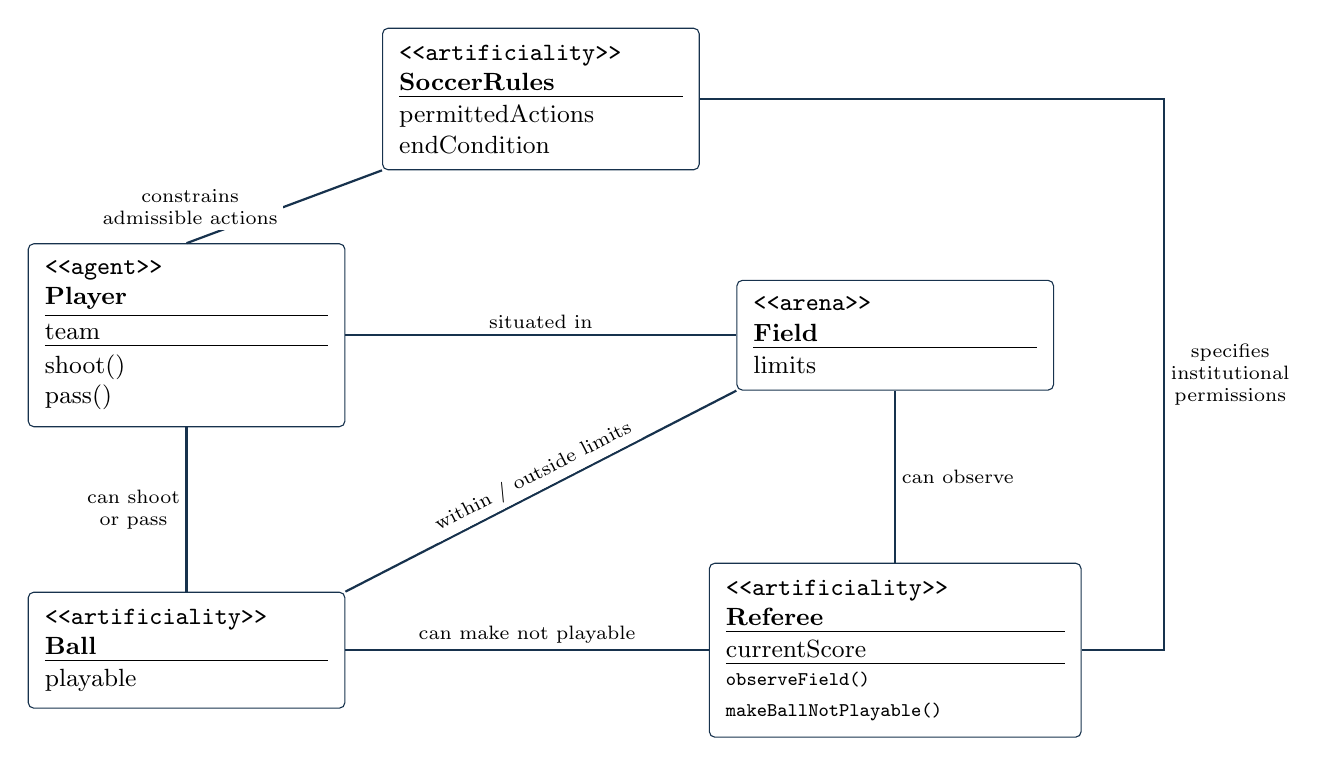
\begin{tikzpicture}
\node[entity] (rules) at (0,0) {\rules{1}};
\node[entity] (player) at (-4.5,-3) {\player{1}{1}};
\node[entity] (field) at (4.5,-3) {\field{1}};
\node[entity] (ball) at (-4.5,-7) {\ball{1}};
\node[entity,text width=43mm] (ref) at (4.5,-7) {\referee{1}{1}};
\draw[rel] (rules.south west)--node[lab,left]{constrains\\admissible actions}(player.north);
\draw[rel] (rules.east)-- ++(5.9,0) |- node[lab,pos=.25,right]{specifies\\institutional\\permissions}(ref.east);
\draw[rel] (player.east)--node[lab,above]{situated in}(field.west);
\draw[rel] (player.south)--node[lab,left]{can shoot\\or pass}(ball.north);
\draw[rel] (ball.north east)--node[lab,sloped,above]{within / outside limits}(field.south west);
\draw[rel] (ref.north)--node[lab,right]{can observe}(field.south);
\draw[rel] (ref.west)--node[lab,above]{can make not playable}(ball.east);
\end{tikzpicture}
\end{center}
\textbf{Updated description.} Players, identified by team, are situated in the field and can shoot or pass the ball. The ball has a playable state and can be within or outside field limits. The referee records scores, can observe the field, and can make the ball not playable. SoccerRules specifies permitted player actions and institutional permissions for the referee, together with an end condition. The diagram does not yet prescribe how these capacities are enacted.

\heading{Stop: compare, revise, and accept provisionally}
Read the description and inspect the LUL. \textbf{They should express the same model.} It represents what you wrote, not what you intended or silently assumed. Remove unnecessary text or structure; add or clarify what is missing. Check that the desired result has not been prescribed.

Once the representation is sufficiently explicit and useful for attempting the first process specification, accept it as \textbf{$O_0$}. It may still be incomplete or mistaken. This is our stopping point before constructing \textbf{$FC_0[O_0]$}, the first process specification. If that work exposes a gap, return to the ontology.
\newpage
\heading{After accepting $O_0$: construct $FC_0[O_0]$}
Only now do we move from WHAT IS to HOW. The following is a deliberately incomplete first flowchart for the provisionally accepted ontology. It is a diagnostic proposal, not a complete executable specification. Its arrows indicate process order, unlike the relation lines in LUL.

This initial FC restricts player choice to the represented permitted actions, shoot and pass. That is an explicit compliance assumption, not a general property of institutional rules. We do not use ``close to goal'' here: this ontology contains no Goal class or proximity relation. After a pass, the flow returns directly to action selection, as in our initial sketch.

\begin{center}
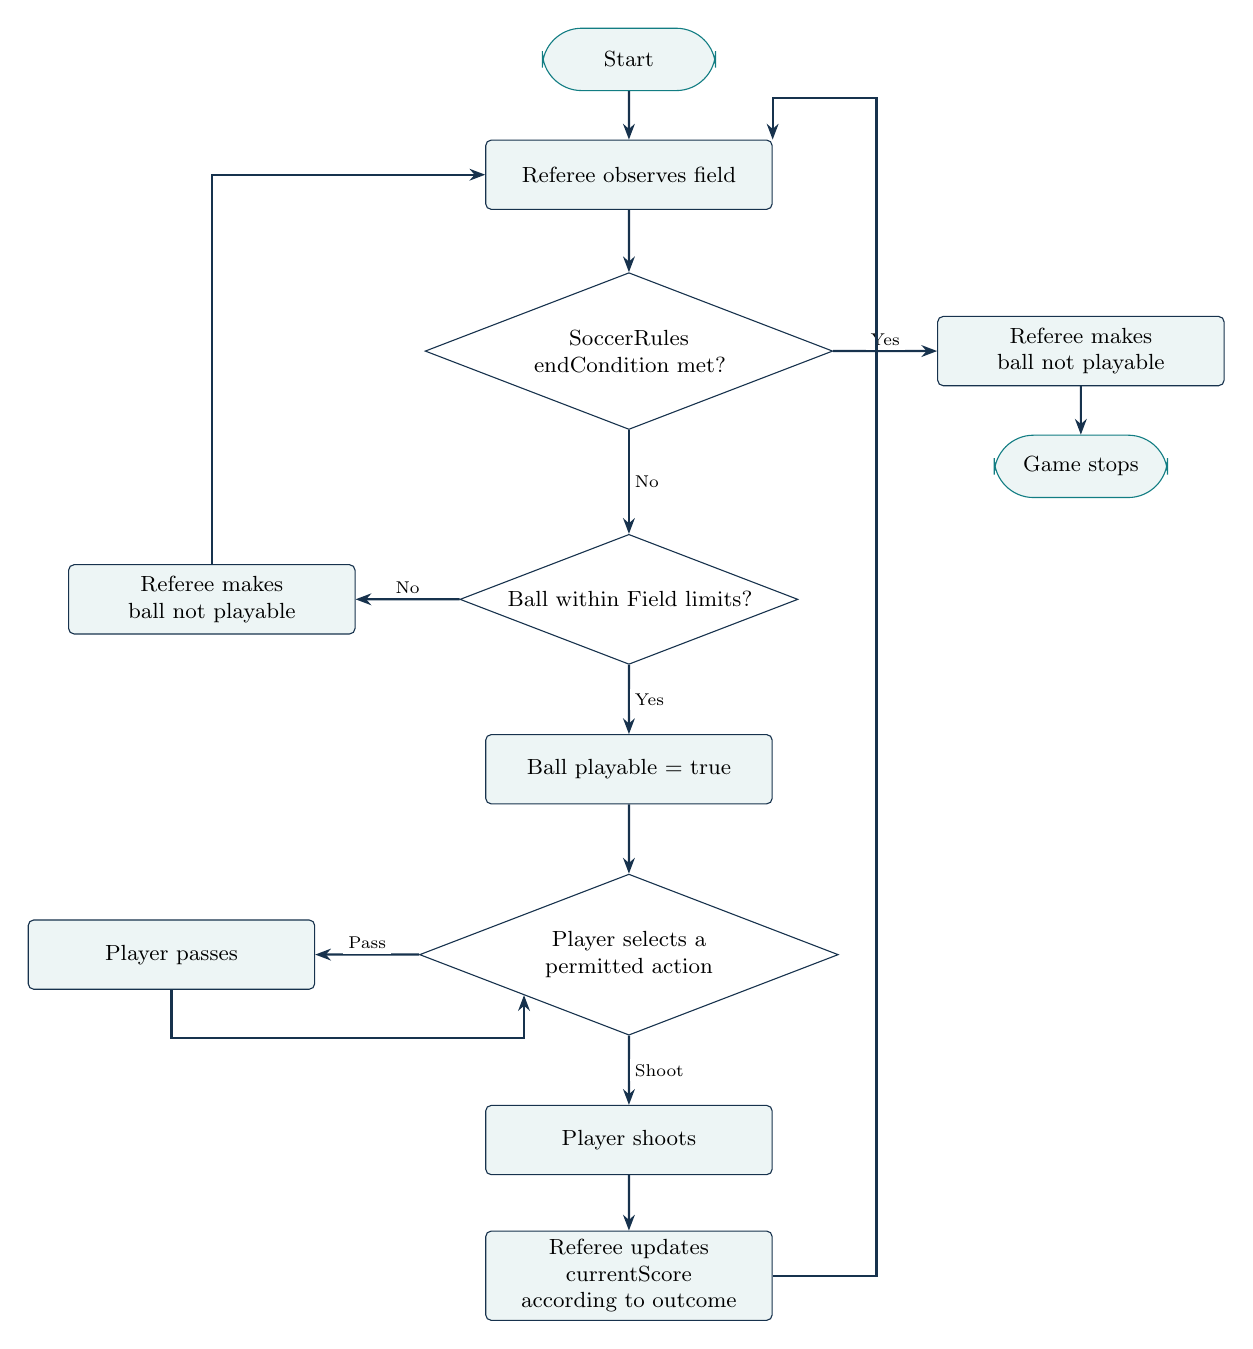
\begin{tikzpicture}[
 scale=.88,transform shape,
 proc/.style={draw=ink,rounded corners=2pt,fill=pale,text width=39mm,minimum height=10mm,align=center,font=\small},
 choice/.style={diamond,aspect=2.6,draw=ink,text width=38mm,inner sep=2pt,align=center,font=\small},
 term/.style={draw=teal,rounded corners=5mm,fill=pale,minimum width=25mm,minimum height=9mm,font=\small},
 arr/.style={-{Stealth[length=2mm]},draw=ink,thick}]
\node[term] (start) {Start};
\node[proc,below=7mm of start] (observe) {Referee observes field};
\node[choice,below=9mm of observe] (endq) {SoccerRules\\endCondition met?};
\node[proc,right=15mm of endq] (endball) {Referee makes ball not playable};
\node[term,below=7mm of endball] (stop) {Game stops};
\node[choice,below=15mm of endq] (bounds) {Ball within Field limits?};
\node[proc,left=15mm of bounds] (out) {Referee makes ball not playable};
\node[proc,below=10mm of bounds] (play) {Ball playable = true};
\node[choice,below=10mm of play] (action) {Player selects a permitted action};
\node[proc,left=15mm of action] (pass) {Player passes};
\node[proc,below=10mm of action] (shoot) {Player shoots};
\node[proc,below=8mm of shoot] (score) {Referee updates\\currentScore\\according to outcome};
\draw[arr] (start)--(observe);
\draw[arr] (observe)--(endq);
\draw[arr] (endq)--node[lab,above]{Yes}(endball);
\draw[arr] (endball)--(stop);
\draw[arr] (endq)--node[lab,right]{No}(bounds);
\draw[arr] (bounds)--node[lab,above]{No}(out);
\draw[arr] (out.north)|-(observe.west);
\draw[arr] (bounds)--node[lab,right]{Yes}(play);
\draw[arr] (play)--(action);
\draw[arr] (action)--node[lab,above]{Pass}(pass);
\draw[arr] (pass.south)-- ++(0,-7mm) -| (action.south west);
\draw[arr] (action)--node[lab,right]{Shoot}(shoot);
\draw[arr] (shoot)--(score);
\draw[arr] (score.east)-- ++(15mm,0) |- ([yshift=6mm]observe.north east) -- (observe.north east);
\end{tikzpicture}
\end{center}

\textbf{Read this as a first process proposal.} ``Updates currentScore'' does not mean every shot scores. It exposes a question we have not answered: how is the outcome recognized? The flow names this step without yet specifying its mechanism. It also introduces score updating and restoration of play without matching declared methods. Those mismatches are left visible for diagnosis, not accepted as a finished implementation.

\newpage
\heading{What FC helps us discover}
We thought carefully while preparing LUL: selecting entities, assigning roles, adding state and methods, and making relations explicit. That work was necessary. It did not guarantee that we had specified everything needed for the model to operate.

When we construct FC, we must connect those commitments into a process. We ask what happens next, which condition is checked, and what changes. \textbf{This is when missing parts become visible.} The purpose of this first flowchart is therefore also diagnostic: it helps us inspect the ontology we have just accepted provisionally.

\heading{Check the bridge from LUL to FC}
For every FC process, identify the method and state it uses. For every decision, identify the information that makes the condition evaluable. For every interaction, identify the corresponding relation. Then ask what CLOCK contributes: activation, order, repetition, synchronization, and termination.

In this proposal, ``within limits'' lacks an explicit ball position; score updating lacks a declared method and goal-recognition mechanism; restoring play lacks a restart procedure. The passing loop bypasses observation and stopping checks. Some gaps require changes to LUL; others concern FC order. The final TO-DO explores these differences through explicit WHAT IF questions.

\heading{Return to LUL when the question requires it}
Not every question requires a new class. A missing execution order or choice rule may be resolved in FC. Missing state, methods, or relations require a revision to LUL as well. For example, if dismissals matter to our question, we may need to represent player eligibility and the institutional capacity to change it. We do not add those features here merely because real soccer contains them.

Keep the current $O_0$ as our explicit starting point. Record the gaps, decide which matter to the explanatory question, and revise the description, LUL, and FC together when needed. A substantive revision may become $O_1$.
\[
\underbrace{O_0}_{\text{WHAT IS}}
\longrightarrow
\underbrace{FC_0[O_0]}_{\text{HOW}}
\xrightarrow{\text{reveals missing commitments}}
\text{review }O_0.
\]
\textbf{Accepting $O_0$ is a working decision, not a claim of completeness.} We have reached a point where attempting the flow teaches us what else the model needs. The rule still holds: do not build the result; let it emerge from the specified mechanisms.


\newpage
\section*{Required TO-DO: WHAT IF?}
\addcontentsline{toc}{section}{Required TO-DO: WHAT IF?}
\textbf{Always end your homework with a TO-DO in the form of WHAT IF thought experiments.} Divide it into the two sections below. For each question, write a short tentative answer, explain what could improve, and reflect on what could break or require reconsideration. The worked responses here are hypotheses, not results or instructions to implement every change. Adapt them to your own model and add questions it raises.

These sections distinguish the starting point of a question, not isolated compartments: an ontological change can force a new FC, and an FC change can expose missing state, methods, or relations. Keep the previous version for comparison.

\subsection*{1. Ontological WHAT IFs --- Revisiting WHAT IS}

\heading{WHAT IF the referee becomes an agent?}
\textbf{Tentative answer.} Move the referee from the stipulated service in $A_{3s}$ to $A_1$. Represent its information, observations, interpretation, and enforcement decisions. The officiating role and prescriptions remain in $A_{3s}$; observation and authority links remain A4 relations.

\textbf{What could improve?} We could investigate missed incidents, different interpretations, or player responses to enforcement rather than assume a uniform automatic response.

\textbf{What could break or require reconsideration?} The current FC assumes automatic observation and enforcement. Its timing and information assumptions must be reconsidered. Remove the old service to avoid duplicate sanctions. Earlier findings may not survive; becoming an agent does not guarantee a better explanation.

\heading{WHAT IF players have an eligibility state?}
\textbf{Tentative answer.} Add a state such as eligible/ineligible to Player if dismissals matter. Specify the institutional grounds and a method that can change eligibility, then revise FC so only eligible players can act.

\textbf{What could improve?} Dismissal could have consequences distinct from temporarily stopping the ball. We could investigate how exclusions affect coordination.

\textbf{What could break or require reconsideration?} Existing player-selection and passing procedures may still choose an ineligible player. Possession and restart arrangements would need review. Simply adding a field to the class changes nothing unless dynamics use it.

\newpage
\heading{WHAT IF possession is explicitly represented?}
\textbf{Tentative answer.} Represent who controls the ball, for example through a ball-holder relation, allowing a no-holder state where appropriate. Decide whether redundant player flags are needed. State explicitly when possession can change.

\textbf{What could improve?} We could identify the acting player, receivers, and turnovers, and investigate sequences of possession.

\textbf{What could break or require reconsideration?} The FC currently selects an unspecified player. It must respect possession and resolve conflicting claims. Duplicated holder information could become inconsistent. A completed pass need not occur after every attempted pass.

\heading{WHAT IF goal recognition becomes explicit?}
\textbf{Tentative answer.} Represent the distinctions needed to recognize a goal: perhaps goal regions in Field, relevant ball position, and a recognition and score-update method. A new Goal class is one option, not an automatic requirement.

\textbf{What could improve?} The score would follow a specified event rather than an unexplained ``outcome.'' The model could distinguish shots from goals.

\textbf{What could break or require reconsideration?} Shooting, spatial relations, team attribution, and restarts need consistent definitions. An aggregate goal probability and a geometric recognition rule could double-count the same event if both remain active.

\heading{WHAT IF we remove the referee?}
\textbf{Tentative answer.} Remove the referee class and reconsider every method, state, and relation assigned to it. If score recording or automatic stopping is still needed, explicitly justify its new location. An alternative model might investigate self-enforcement, but would need mechanisms for it.

\textbf{What could improve?} A comparison could reveal which patterns depend on centralized enforcement, or simplify a question for which referee representation is unnecessary.

\textbf{What could break or require reconsideration?} Observation, score storage, and stopping currently rely on that class. Leaving those functions silently in the code would not establish that enforcement had disappeared. Removal can require extensive re-specification elsewhere.

\newpage
\subsection*{2. Flowcharting WHAT IFs --- Revisiting HOW}

\heading{WHAT IF observation and stopping checks occur after every action?}
\textbf{Tentative answer.} Route both pass and shoot branches back through observation and the stopping check. Define what one action means for CLOCK and how the institutional end condition is evaluated.

\textbf{What could improve?} Repeated passes would no longer bypass the opportunity to stop play. The schedule would be more explicit and easier to inspect.

\textbf{What could break or require reconsideration?} More frequent checks can change available actions and trajectories. A time-based end condition also needs elapsed time and a defined time increment; rerouting arrows alone does not supply them. Compare schedules rather than assume they are behaviorally equivalent.

\heading{WHAT IF a pass resolves possession before another player acts?}
\textbf{Tentative answer.} Determine the pass outcome, update the holder, and only then select the next actor. This requires the possession commitment discussed in the ontological TO-DO; a failed or intercepted pass needs an explicit resolution rule.

\textbf{What could improve?} Action order would follow a defined transfer of control. Passing sequences and turnovers would become interpretable.

\textbf{What could break or require reconsideration?} The original direct loop is no longer adequate. Player-selection rules, action opportunities, and time advancement may change. Resolving all passes as successful would silently impose an additional assumption.

\heading{WHAT IF restarting play is a separate process?}
\textbf{Tentative answer.} After play stops, determine restart authorization, ball placement, and the next actor before restoring playable status. Declare missing state, methods, and relations in LUL where necessary.

\textbf{What could improve?} The model would explain how an out-of-bounds ball returns to play, rather than repeatedly rechecking an unchanged condition.

\textbf{What could break or require reconsideration?} The unconditional ``playable = true'' update must be replaced. Restart rules can alter possession and advantage; they must not operate after the match has ended. A method for placing the ball cannot be assumed if none has been specified.

\newpage
\heading{WHAT IF players decide simultaneously rather than sequentially?}
\textbf{Tentative answer.} Let eligible actors form proposals from a shared state, resolve conflicts, and commit updates at a defined synchronization point. Shared-state decisions do not require parallel computer hardware.

\textbf{What could improve?} We could investigate whether conclusions depend on who happens to act first, or represent concurrent opportunities more appropriately.

\textbf{What could break or require reconsideration?} Several actors may claim the ball or propose incompatible actions. Immediate sequential updates cannot simply be retained. Proposal storage, conflict-resolution methods, and access to information may require LUL revisions as well as a different FC.

\heading{WHAT IF we slightly change the initial player positions?}
\textbf{Tentative answer.} Once position is explicitly represented and the model can run, repeat the \emph{same model and FC} with nearby starting configurations. Record the perturbation, hold other settings fixed, and use multiple stochastic replications where relevant. This is an initialization and experimental question attached to the FC, not necessarily a new ontology.

\textbf{What could improve?} We could assess whether a claimed pattern is stable across nearby starting conditions or depends strongly on a particular configuration.

\textbf{What could break or require reconsideration?} A conclusion from one initialization may no longer hold. Differences may reflect stochastic variation, thresholds, or implementation errors; one divergent pair of runs does not establish chaos. Investigate initial-condition sensitivity within each version separately from comparisons between model versions.

\heading{Close the TO-DO with a reasoned next step}
Choose which WHAT IF deserves investigation next and explain why. You may decide to retain the current model, remove something, revise its ontology, alter its schedule, or conduct a comparison before editing it. Do not describe a tentative answer as an observed result.

A small revision may substantially alter behavior, including sensitivity to initial conditions. That possibility must be tested rather than presumed. Keep earlier versions so that changes in representation, dynamics, and starting conditions can be distinguished.
\[
\boxed{\text{Progressive construction is re-specification, not accumulation.}}
\]
\end{document}

